%!TEX root = ../dissertation.tex

\chapter{Introduction} \label{cha:introduction}

As industrial robots become faster, smarter, and cheaper, more and more companies are beginning to integrate this technology in conjunction with their workforce. 
Nowadays, robots have a range of applications that cover many different areas. These applications are no longer limited in structured environments, where the robot behavior could be directly specified by a human.
Where early robots blindly followed the same path, and later iterations used lasers or vision systems to detect the orientation of parts and materials, the latest generations of robots can integrate information from multiple sensors and adapt their movements in real time. They can also make use of more powerful computer technology and big data–style analysis. \\
Advances in artificial intelligence and sensor technologies allow robots to cope with a far greater degree of task-to-task variability. However, their ability to adapt to different tasks is still a long way from a general level of adaptability. 
Until now, for example, every industrial robot is designed with a specific purpose. Even the most advanced robots, which exploit Neural Networks (NN) and Artificial Intelligence (AI), are unable to easily learn a new task.
It is necessary to design the AI architecture carefully and, to be successful, people must stop misusing the term AI. This term is used by generalizing those that are the three types of AI: Narrow-AI, General-AI, and Super-AI. The distinction between them is the key to technological progress, especially in the robotic field. 


\section{Artificial Intelligence}\label{sec:ai}

The following is a brief description of these three AI types, the Articles \cite{davidson_2019, edi_weekly, lawtomated_2020, allan_2018, astute_solutions_2020} talk more about this. 

\begin{enumerate}
\item Narrow-AI: \\
Current AI technologies fall under the Artificial Narrow Intelligence (ANI or Narrow-AI) category, which means they are very good at only one or a few closely related tasks. This type of AI has a limited range of abilities, specifically designed for a narrow use. It is able to reach a level of performance of a human, and even better, but only within this limited field that is its specialty. Examples of ANI are Siri, Face ID, Google's assistant, self-driving cars and DeepMind's board game playing program \cite{bhatia_2021}. This is the only form of AI that has been developed so far.

\item General-AI: \\
The next step after ANI is Artificial General Intelligence (AGI or General-AI), much more similar to human intelligence and not focused on specific tasks. It would be similar to a human mind and, in theory, it should be able to think and function like it, being able to make sense of different content, understand issues, and decide what is best in a complex situation. 
AGI hasn’t been achieved yet. There isn't the technical capacity of producing something as complex yet, and there is also no certain knowledge of how the human brain actually works either. 
AGI is a relatively logical and rational future though, and it could be attained at some point if humans develop their knowledge and understanding, as well as technical skills to a high enough level. \\
An overview of AGI, including important reflections written by Ben Goertzel, can be found in \cite{goertzel_AGI}.

\item Super-AI: \\
The final step that AI could hypothetically achieve is Artificial Super Intelligence (ASI or Super-AI). This can only happen when AGI will be achieved and computers will be able to learn autonomously at a very fast rate and exponentially improve their capabilities on their own, without human intervention. At this stage, AI would be capable of vastly outperforming the best human brains in practically every field. The evolution from AGI to ASI would in theory be fast, since AGI would allow computers to “think” and exponentially improve themselves once they are able to really learn from experience and by trial and error \cite{dambrot2019symbiotic}.
\end{enumerate}

The most important differences, easily deduced from the definitions above, are between ANI and AGI, partly because ASI will only be considered when AGI exists. 
The timing forecasts and the difficulties of that step can be found in \cite{995_experts_opinions}. \\
These differences immediately lead into much wider contexts than industry, as AGI seems focused on complex environments such as real-world and human-computer interaction. \\
However, using an AGI system in an industrial setting can have many benefits, as explained in the next section.


\section{Motivation and Challenges}\label{sec:motivation} %% TODO: Magari aggiungi un ref a opencog advantages

In order to design a general purpose planning system, a declarative language for formalizing the domain first needs to be selected, followed by the selection of a suitable solver which supports this language. Many different factors affect this selection process.
For this reason, careful consideration needs to be given to the selection of language and solver \cite{DBLP:journals/corr/abs-1804-08229}.
However, in general, these considerations tend, either voluntarily or involuntarily, to restrict the possible domains or to force the description of the domain using only the features supported by the solver.
In this project, it is proposed to use an AGI-Based system for Task Planning, to generalise as much as possible the domains and the problems to be solved.
Consequently, the aim of this proposal is to obtain a system capable of solving any manipulation problem that has a domain with four specific actions: Pick, Place, Stack and Unstack (see Section \ref{sec:domain_atomese}).  
That is, a Task Planning system developed starting from the classical blocks world problem, but which is also strongly oriented towards its expansion (e.g., to easily add further actions or more detailed domain description), and from which the following features can be obtained:

\begin{itemize}
	\item Having a general knowledge base for the robot, which can be shared with other ones;
	\item Use the robot(s) to cover multiple and complex tasks;
	\item Make cooperation with humans operators and encourage learning from them;
	\item Robot(s) is robust to changes in the environment, its state, and its task;
	\item Easier implementation of new modules and their merge into the system;
	\item Not only maintain, but rather exploit, existing Narrow-AI systems as modules of the AGI system to take advantage of their potential and allow interaction between them in a \enquote{single} large knowledge base.
\end{itemize}

For this project, one of the proto-AGI\footnotemark{} systems currently under research is used, which proposes a concrete system that demonstrates the feasibility of the concepts just listed, but aims at a much higher purpose. Being able to go into new situations, understand them and create new patterns of behaviour based on what has been learned. This means being able to deal with situations of a radically different nature from those that existed at the time of its creation. \\
\footnotetext{Any current theoretical or practical concept about AGI falls into a category that is called proto-AGI for now. However, in this paper the two terms are considered interchangeable.}

There are several projects and researches that want to achieve the AGI goal. One of these is the Elon Musk and Sam Altman's OpenAI Project. 
Its mission is to ensure that AGI, intended as highly autonomous systems that outperform humans at most economically valuable work, benefits all of humanity.
OpenAI is focused on Deep Neural Networks for almost all projects such as OpenAI Codex, its AI system that translates natural language to code \cite{DBLP:journals/corr/abs-2107-03374}, CLIP (Contrastive Language-Image Pre-Training) a general-purpose vision system, which is a Neural Network trained on a variety of image-text pairs \cite{DBLP:journals/corr/abs-2103-00020} and one of the most important: Generative Pre-trained Transformer 3 (GPT-3). This is an autoregressive language model that uses Deep Learning to produce human-like text \cite{DBLP:journals/corr/abs-2005-14165}. With over 175 billion parameters, it is the largest Neural Network ever created \cite{romero_2021}. \\
Although OpenAI is well-funded and achieving excellent results, there is a second AGI-oriented project that is noteworthy: the Open Cognition (OpenCog) project. It was formally launched in 2008, initially by open sourcing code. A key initial motive was to provide a software platform for exploring a specific (integrative, cross-paradigm) approach to AGI formulated by project cofounder Ben Goertzel. However, the software system has since been used to explore a variety of other AGI ideas as well, and it has also been used as the foundation of several commercial software services (e.g., in bioinformatics, financial prediction and natural language processing). This is the system on which this project is based. \\
The reason for this choice, the preference of OpenCog over OpenAI, lies in the approach to solving the AGI problem.\\
As mentioned above, OpenAI appears to be based on the general plan of starting from current Deep Neural Network tech, applying and extending it in various interesting and valuable ways, and in this way moving incrementally toward AGI without that much of a general plan or model of the whole AGI problem.\\
On the other hand, OpenCog is founded based on a comprehensive model of human-like general intelligence, and a comprehensive overall plan for getting from here to human-level AGI. Thus, it has an integrative approach in which multiple different sorts of AI algorithms (Deep Neural Networks, Probabilistic Logic Theorem Proving, Evolutionary Learning, Concept Blending, etc.) operate together on a common representational substrate.
It is not about building more accurate classification algorithms, or more efficient computer vision systems, or better language processing or boutique information retrieval algorithms, diagnosing diseases, answering trivial questions or driving a car, etc. It is concerned with generic intelligence and the inter-related cognitive processes it entails. It is about making software that perform specific tasks, using structures and processes that appear capable of being extended to more and more general tasks.
The OpenCog system is explained in detail later, in the Chapter \textbf{\ref{cha:opencog_system}}. \\
OpenAI and OpenCog are two distinct ways, both valid. However, we believe that the AGI architecture shouldn't be based on Neural Networks, both because of the general problems as in \cite{323037}, but especially for the following reasons (Figure \ref{fig:disadvantages_nn}):

%Vengono delineati alcuni dei problemi specifici che l'autore ha dovuto affrontare nell'utilizzo delle reti neurali in diverse aree applicative. Riguardano la giustificazione dell'uso delle reti neurali: l'apparente natura ad hoc del metodo; la mancanza di dati di formazione sufficienti; la mancanza di una procedura di convalida accettabile; la necessità di mettere in relazione i pesi della rete con i parametri fisici; le diffuse disparità nei tempi di formazione (tempi di apprendimento) nella risoluzione di problemi apparentemente semplici; la necessità di progressi nell'area dell'implementazione dell'hardware; la necessità di sviluppare sistemi di controllo adattativi basati su prototipi biologici e la necessità di una procedura di sintesi nella ricerca sulle reti neurali.

\begin{itemize}
	\item A huge amount of data is required. \\
Figure \ref{fig:nn_data_process} shows annual data growth versus growth in CPU processing power. The gap leads one to think that as the data required for NNs increases, hardware technology must be improved.
	\item Adversarial Examples problem: it is a way to deceive almost all AI classifiers easily. \\
Figure \ref{fig:adversarial_examples} is an illustration of machine learning adversarial examples. Studies have shown that by adding an imperceptibly small, but carefully designed perturbation, an attack can successfully lead the machine learning model to making a wrong prediction. For more information see \cite{42503, DBLP:journals/corr/abs-1905-10615, 7467366, goodfellow_2020}.
	\item The cost: training GPT-3, for example, would have an estimated cost between \$4.6 and \$12 million \cite{dickson_2020, wiggers_2021}. \\
Figure \ref{fig:nn_development_process} gives a general idea of a NN development process .  
	\item Neural Networks as black box: the best-known disadvantage of Neural Networks is their “black box” nature. It means that, while it can approximate any function, studying its structure won't give any insights on the structure of the function being approximated. More details in \cite{DBLP:journals/corr/abs-1911-12116}. 
\end{itemize}

\begin{figure}
\begin{subfigure}{.5\linewidth}
	\centering
	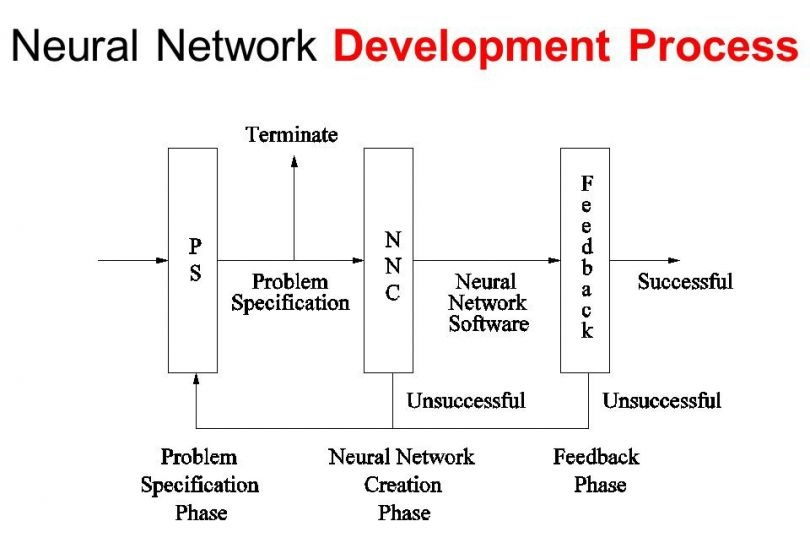
\includegraphics[width=\textwidth]{figures/Magistrale/02 - neural-networks-development-process}
	\caption{Neural Network development process. \\Image source: \cite{img02}.
	\label{fig:nn_development_process}}
\end{subfigure}%
\begin{subfigure}{.5\linewidth}
	\centering
	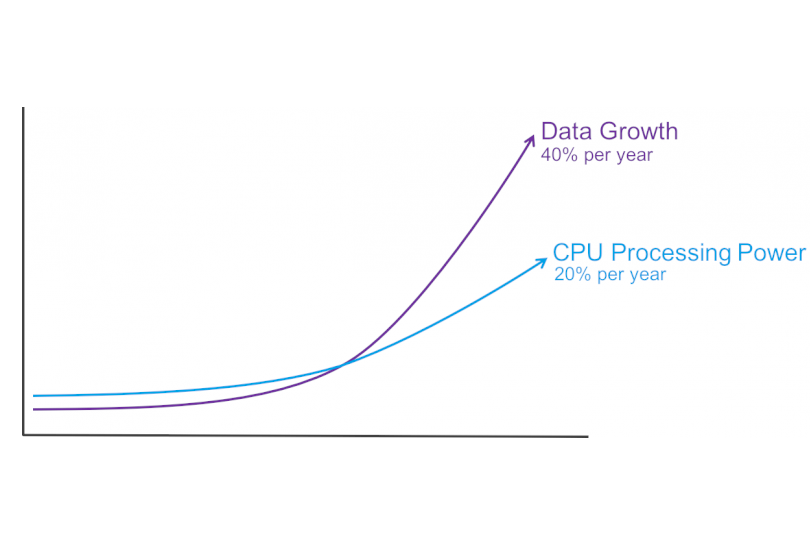
\includegraphics[width=\textwidth]{figures/Magistrale/03 - neural-networks-data-process}
	\caption{Neural Network data process. \\Image source: \cite{img03}.
	\label{fig:nn_data_process}}
\end{subfigure}\\[5ex]
\begin{subfigure}{\linewidth}
	\centering
	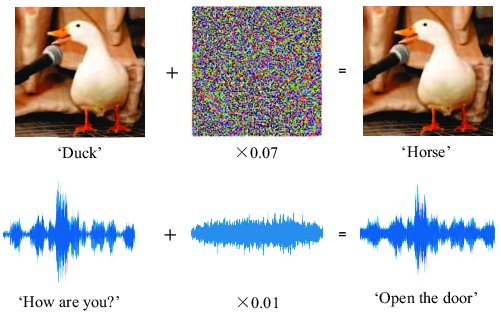
\includegraphics[width=0.7\textwidth]{figures/Magistrale/05 - adversarial-examples}
	\caption{Adversarial Examples. \\Image source: \cite{img05}.
	\label{fig:adversarial_examples}}
	\end{subfigure}
\caption{Some disadvantages of Neural Networks.}
\label{fig:disadvantages_nn}
\end{figure} 


The disadvantages of an NN-based approach like OpenAI have been mentioned. Now, to understand the advantages of a human-like approach like OpenCog, it is necessary to explain the OpenCog system. Therefore, these advantages are postponed to the Section \ref{sec:opencog_advantages}. \\

\textbf{Update:} OpenAI shuts down robotics team because it doesn't have enough data yet.\\
In June 2021, on a podcast hosted by startup Weights \& Biases, Wojciech Zaremba, co-founder of OpenAI, who led the robotics group confirmed that the company recently broke up the team to focus working on more promising areas of artificial general intelligence research.
Zaremba said: \enquote{There wasn't enough information (lack of training data) on hand to teach the systems to the level of intelligence desired. From the perspective of what we want to achieve, which is to build AGI, I think there was actually some components missing} \cite{wiggers_openai_2021,oitzman_2021,quach_2021}.


\section{Contributions}\label{sec:contributions}

Many tests and attempts have been made to achieve this goal. Together with some members of the OpenCog team, different strategies to solve the problem were analysed\footnotemark{}. The first development attempt was based on Backward Chaining inference strategy (see Section \ref{sec:ure}), but was abandoned due to conceptual and practical problems. Subsequently, the one proposed in this paper was implemented, while the first one was revisited and some solutions to its problems were sketched (Section \ref{sec:future_devel}).
\footnotetext{\url{https://groups.google.com/g/opencog/c/WUOIi1CHqos}}
The main contributions, therefore, correspond to the search for the best way to describe these problems (any manipulation problem that has a domain with the four specific actions) within the AGI-based system and the implementation of a suprasystem using it, which through an algorithm (introduced in Section \ref{sec:bfs_search}) is able to solve these problems.
Since this is an unexplored area of research for the AGI-based system used, a few external modules (i.e., the vision system, for object recognition, and the manipulation system, for interaction with them) were simplified, without loss of generality, to focus on the main objective.  
